\documentclass{SMR}
\usepackage{paralist}

%graphics
\graphicspath{ {/Where/you/keep/your/graphics} }  % <- UPDATE THE PATH

%who and where
\smrtitle{SMR.cls}
\smrauthor{Marcin and Nick}
\smraffiliation{Edinburgh and Glasgow Universities}

\title{Scottish Music Review class file for PDFLaTeX}
\author{Pietryszwski, Marcin \and Bailey, Nick}

\begin{document}

\newcommand{\cmd}[1]{\texttt{\textbackslash #1}}

\maketitle

\begin{abstract}
A class for the Scottish Music Review
\end{abstract}

\section{Section One - comment out if not needed} %section title comes here,
                                                  %comment out if there are
                                                  %no sections in the article 
The usual title, author and date commands given in the preamble
are used to head up the paper, but there's also the smr- varients
which get used in the headers.

If you don't supply them it'll still work, but you'll be warned.

If you supply an smrauthor, you \emph{must} supply an affiliation.

The title is set at the top left of left-hand pages, and the
author above the affiliation at the top right of right-hand pages.

\vspace*{1.0cm}

Here is some text to be formatted followed by a figure of
a Klein Bottle as an example of how graphics are formatted
in this template.

\begin{figure}[h]
\caption{Klein Bottle} %EDIT CAPTION
\centering
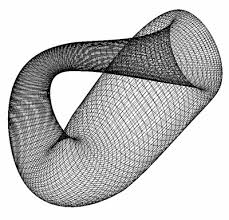
\includegraphics[width=0.5\textwidth]{klein.jpg}
\end{figure}

Here is some text following a figure with a footnote added
to it \footnote{I am a footnote}. Here is an \emph{emphasized text}
followed by \textbf{bold text} which can be used for
\textbf{[Referencing]}

\pagebreak

\subsection{A Subsection} %subsections

Subsections are numbered per section.

\section{A New Section}

This section has its own subsection.

\subsection{Another subsection}

Like this one.

\section{Heavy-duty usage}
\subsection{Music glyphs}
This style requires the lilyglyphs package (spelt
	\textit{lily}%
	\clefGInline[scale=0.8,raise=0.2]%
	\lilyOpticalSize{26}%
	ly\lilyDynamics{p}%
	\lilyOpticalSize{13}%
	\hspace*{0.2ex}\flat[scale=0.9,raise=0.2]%
	\lilyOpticalSize{11}%
	\lilyDynamics{s}) which
enables the use of Lilyponds Emmentaler font in the text. The full documentation
is available on
\href{http://mirrors.ctan.org/macros/luatex/latex/lilyglyphs/documentation/lilyglyphs.pdf}{CTAN}.
Glyphs are included through their names, and most are guessable, but a necessarily abbreviated
crib sheet follows.

\begin{table*}
{\small
\begin{tabular}{r|l l}
\wholeNote & \cmd{semibreve} -- \cmd{wholeNote}\\
\wholeNoteDotted & \cmd{semibreveDotted} -- \cmd{wholeNoteDotted}\\
\halfNote & \cmd{minim} -- \cmd{halfNote}\\
\halfNoteDown & \cmd{minimDown} -- \cmd{halfNoteDown}\\
\halfNoteDotted & \cmd{minimDotted} -- \cmd{halfNoteDotted}\\
\halfNoteDottedDown & \cmd{minimDottedDown} -- \cmd{halfNoteDottedDown}\\
\halfNoteDottedDouble & \cmd{minimDottedDouble} -- \cmd{halfNoteDottedDouble}\\
\halfNoteDottedDoubleDown & \cmd{minimDottedDoubleDown} -- \cmd{halfNoteDottedDoubleDown}\\
\crotchet & \cmd{crotchet} -- \cmd{quarterNote}\\
\crotchetDown & \cmd{crotchetDown} -- \cmd{quarterNoteDown} & etc...\\
\quaver & \cmd{quaver} -- \cmd{eighthNote}\\
\quaverDown & \cmd{quaverDown} -- \cmd{eighthNoteDown} & etc...\\
\semiquaver & \cmd{semiquaver} -- \cmd{sixteenthNote}\\
\semiquaverDown & \cmd{semiquaverDown} -- \cmd{sixteenthNoteDown}\\
\demisemiquaver & \cmd{demisemiquaver} -- \cmd{thirtysecondNote}\\
\demisemiquaverDown & \cmd{demisemiquaverDown} -- \cmd{thirtysecondNoteDown}\\
\threeBeamedQuavers & \cmd{threeBeamedQuavers} & Three beamed quavers\\
\threeBeamedQuaversI & \cmd{threeBeamedQuaversI} & Second dotted\\
\threeBeamedQuaversII & \cmd{threeBeamedQuaversII} & First dotted\\
\threeBeamedQuaversIII & \cmd{threeBeamedQuaversIII} & Second dotted, first short\\
\hline
\clefGInline & \cmd{clefG}, \cmd{clefGInline} & clefs.G\\
\clefFInline & \cmd{clefF}, \cmd{clefFInline} & clefs.F\\
\clefCInline & \cmd{clefC}, \cmd{clefCInline} & clefs.C\\
\hline
\lilyTimeC & \cmd{lilyTimeC} & timesig.C44\\
\lilyTimeCHalf & \cmd{lilyTimeCHalf} & timesig.C22\\
\lilyTimeSignature{7}{8} & \cmd{lilyTimeSignature\{7\}\{8\}}\\
\lilyTimeSignature{3 + 4}{4 + 8} & \cmd{lilyTimeSignature\{3 + 4\}\{4 + 8\}}\\
\hline
\natural & \cmd{natural} & accidentals.natural\\
\sharp & \cmd{sharp} & accidentals.sharp\\
\flat & \cmd{flat} & accidentals.flat\\
\flatflat & \cmd{flatflat} & accidentals.flatflat\\
\hline
\wholeNoteRest & \cmd{wholeNoteRest} & Whole Note Rest\\
\wholeNoteRestDotted & \cmd{wholeNoteRestDotted} & DottedWhole Note Rest\\
\halfNoteRest & \cmd{halfNoteRest} & Half Note Rest\\
\halfNoteRestDotted & \cmd{halfNoteRestDotted} & Dotted Half Note Rest\\
	\halfNoteRestDotted\lilyPrintMoreDots & 
	\cmd{halfNoteRestDotted}\cmd{lilyPrintMoreDots} &
	Example of Double Dotted Rest\\
\crotchetRest & \cmd{crotchetRest} & Crotchet Rest\\
\crotchetRestDotted & \cmd{crotchetRestDotted} & Dotted Crotchet Rest\\
\quaverRest & \cmd{quaverRest} & Quaver Rest\\
\quaverRestDotted & \cmd{quaverRestDotted} & Dotted Quaver Rest\\
\semiquaverRest & \cmd{semiquaverRest} & Semiquaver Rest\\
\semiquaverRestDotted & \cmd{semiquaverRestDotted} & Dotted Semiquaver Rest\\
\hline
\lilyDynamics{f} & \cmd{lilyDynamics\{f\}} & forte\\
\lilyDynamics{p} & \cmd{lilyDynamics\{p\}} & piano\\
\lilyDynamics{m} & \cmd{lilyDynamics\{m\}} & mezzo-\\
\lilyDynamics{r} & \cmd{lilyDynamics\{r\}} & rin-\\
\lilyDynamics{s} & \cmd{lilyDynamics\{s\}} & s-\\
\lilyDynamics{z} & \cmd{lilyDynamics\{z\}} & -z\\
\end{tabular}
}
\caption{Get-you-started-quick crib sheet for music glyphs in the body text}
\end{table*}



%a separate section for bibliography
You will find the bibliography on the next page.
\vfill\pagebreak


\section*{Bibliography}

\end{document}
